%----------------------------------------------------------------------------------------
%	PACKAGES AND THEMES
%----------------------------------------------------------------------------------------
\documentclass{beamer}
\mode<presentation> {
\usetheme{Berlin}
}
\AtBeginSection[]{
  \begin{frame}
  \vfill
  \centering
  \begin{beamercolorbox}[sep=8pt,center,shadow=true,rounded=true]{title}
    \usebeamerfont{title}\insertsectionhead\par%
  \end{beamercolorbox}
  \vfill
  \end{frame}
}
\usepackage{graphicx} % Allows including images
\usepackage{booktabs} % Allows the use of \toprule, \midrule and \bottomrule in tables
\usepackage{epigraph}
\setlength\epigraphwidth{8cm}
\setlength\epigraphrule{0pt}
\patchcmd{\epigraph}{\@epitext{#1}}{\itshape\@epitext{#1}}{}{}
\usepackage{listings}
%----------------------------------------------------------------------------------------
%	TITLE PAGE
%----------------------------------------------------------------------------------------
\titlegraphic{
\includegraphics[width=3.5cm]{photo/logo}}

\title{IT-Project \\ Autonomously driving Remote Control Car} % The short title appears at the bottom of every slide, the full title is only on the title page
\author{Bohnstedt Timo ,
      L\"ohr Tim and Palpanis Ionannis\\%
      } 
\institute[Computer Science| Prof. Dr. Florian Gallwitz] % Your institution as it will appear on the bottom of every slide, may be shorthand to save space
{
Georg Simon Ohm University of Applied Science\\ % Your institution for the title page
\medskip
\textit{IT Project Presentation} 
}
\date{\today} % Date, can be changed to a custom date
%----------------------------------------------------------------------------------------
\begin{document}

\begin{frame}
\titlepage % Print the title page as the first slide
\end{frame}
%----------------------------------------------------------------------------------------
\begin{frame}
\frametitle{Overview} % Table of contents slide, comment this block out to remove it
\tableofcontents % Throughout your presentation, if you choose to use \section{} and \subsection{} commands, these will automatically be printed on this slide as an overview of your presentation
\end{frame}
%
%----------------------------------------------------------------------------------------
%	PRESENTATION SLIDES
%----------------------------------------------------------------------------------------
%------------------------------------------------
\section{Background}
%------------------------------------------------
%
\begin{frame}
\frametitle{Background}
\begin{center}
"We can build these models, but we don't know how they work."  \textup{---Joel Dudley}, MITs Technology Review
\end{center}
\begin{figure}
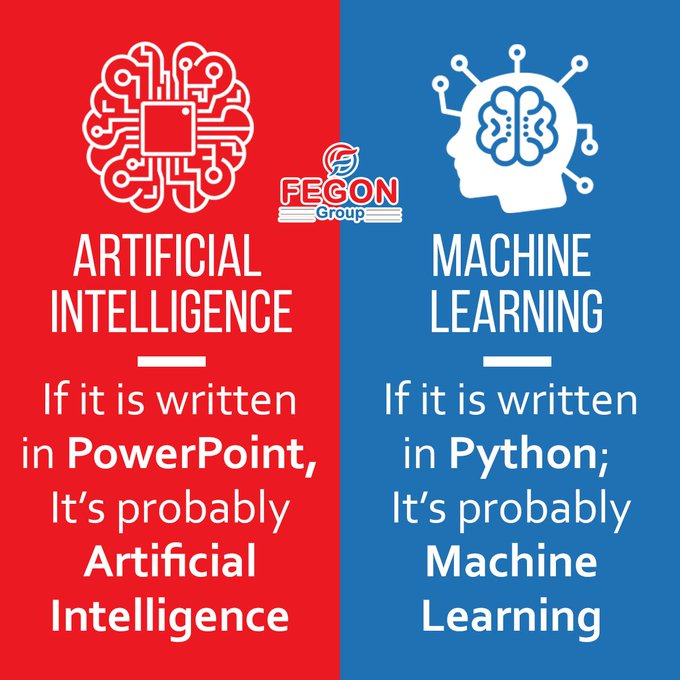
\includegraphics[width=0.4\linewidth]{photo/aivsml}
\end{figure}
\end{frame}
%
%------------------------------------------------
\section{Literature Survey}
%---------------------------------------------
%
\begin{frame}
\frametitle{The Level of autonomously driving Cars - Part I}
\begin{block}{Level 0}
No Automation
\begin{itemize}
\item Driven by a human
\end{itemize}
\end{block}
\begin{block}{Level 1}
Driver Assistance
\begin{itemize}
\item Steering into the middle of the lane
\item Breaking tires when the distance to the car in front is to close
\item Just one system at a time 
\end{itemize}
\end{block}
\end{frame}
%
%------------------------------------------------
%
\begin{frame}
\frametitle{The Level of autonomously driving Cars - Part II}
\begin{block}{Level 2}
Partial Automation
\begin{itemize}
\item A computer programm drives the car (accelerating and decelerating)
\item The human is responsible and still in control
\end{itemize}
\end{block}
\begin{block}{Level 3}
Conditional Automation
\begin{itemize}
\item Like above but the computer looks over the environment as well
\item The computer is able to handle easy  standard scenarios
\item Example: Google Waymo self-driving car 
\end{itemize}
\end{block}
\end{frame}
%
%------------------------------------------------
%
\begin{frame}
\frametitle{The Level of autonomously driving Cars - Part III}
\begin{block}{Level 4}
High Automation
\begin{itemize}
\item The computer can handle every situation 
\item Without very special circumstances
\end{itemize}
\end{block}
\begin{block}{Level 5}
Conditional Automation
\begin{itemize}
\item The human is not required to be in the car
\item E.g. it would be possible that cars search for parking lots by themselves
\end{itemize}
\end{block}
\end{frame}
%
%------------------------------------------------
%
\begin{frame}
\frametitle{Reinforcement Learning - Part I}
\epigraph{ " [...] What we want is a machine that can learn form experience."}{--- \textup{ Alan Turing}, 1947}
\begin{figure}
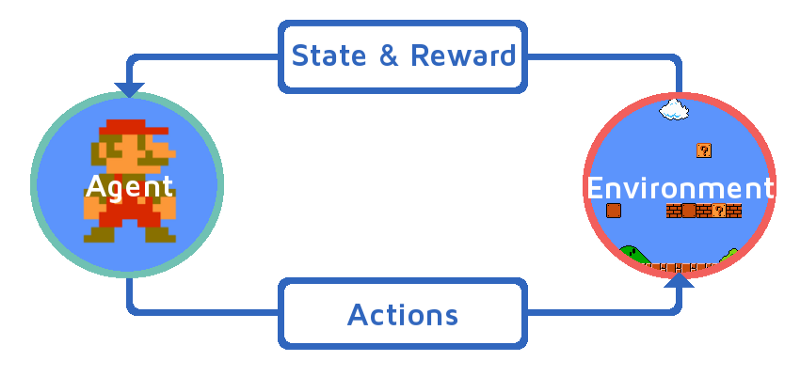
\includegraphics[width=0.6\linewidth]{photo/rl}
\end{figure}
\end{frame}
%
%------------------------------------------------
%
\begin{frame}
\frametitle{Reinforcement Learning - Part II}
\begin{columns}[c] % The "c" option specifies centered vertical alignment while the "t" option is used for top vertical alignment
\column{.45\textwidth} % Left column and width
\textbf{Advantages of unsupervised Learning}
\begin{enumerate}
\item Can find every pattern (unknown objects)
\item Does not need examples, because it can learn from experience ...
\item ... so it is more useful for real-world problems (e. g. autonomous driving)
\end{enumerate}
\column{.5\textwidth} % Right column and width
\begin{block}{DDQN}
Researchers from Google DeepMind (known from achievements at Boardgame GO) developed the Deep Reinforment Learning with Double Q-learning. They showed that reinforcement Learning can be implemented in (Donkey) Cars. 
\end{block}
\end{columns}
\end{frame}
%
%------------------------------------------------
%
\begin{frame}
\frametitle{Reinforcement Learning - Part III}
\begin{figure}
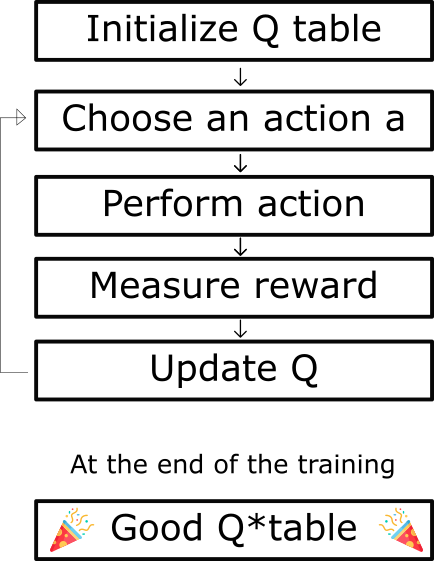
\includegraphics[width=0.4\linewidth]{photo/q}
\end{figure}
\end{frame}
%
%--------------------------------------------------------------------------------------------
%
\begin{frame}
\frametitle{Reinforcement Learning - Part IV}
"The basic idea is to get an Value Q which represents the state s and the action a of an unsupervised machine learning task"\\
\begin{figure}
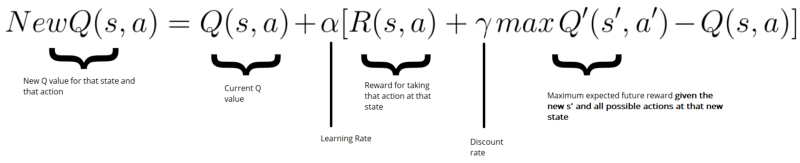
\includegraphics[width=0.9\linewidth]{photo/qformula}
\end{figure}
\end{frame}
%
%--------------------------------------------------------------------------------------------
\section{Hardware}
%----------------------------------------------------------------------------------------
%
\begin{frame}
\frametitle{Remote Control Car}
\begin{itemize}
\item Model car with a servomotor and electronic speed control (ESC)
\item Weights only 1,88kg
\item Easy to attach Raspberry Pi 3B+ and SunFounder Servodriver onto it
\end{itemize}
\begin{figure}
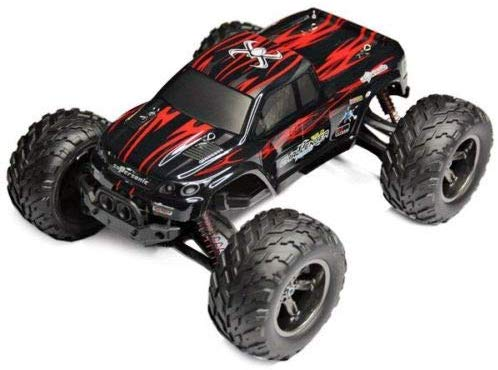
\includegraphics[width=0.4\linewidth]{photo/car.jpg}
\end{figure}
\end{frame}
%--------------------------------------------------------------------------------------------
\begin{frame}
\frametitle{Raspberry Pi 3B+ - Part l}
\begin{itemize}
\item Chosen over NVIDIA's Drive PX for this project, because the weight and power are suiting  better
\item 1.4GHz CPU to apply the Deep Learning to the captured images
\item 16GB SanDisk SD-Card storage with Raspian Stretch Lite
\item Powered through a Powerbank attached onto the RC-Car
\begin{figure}
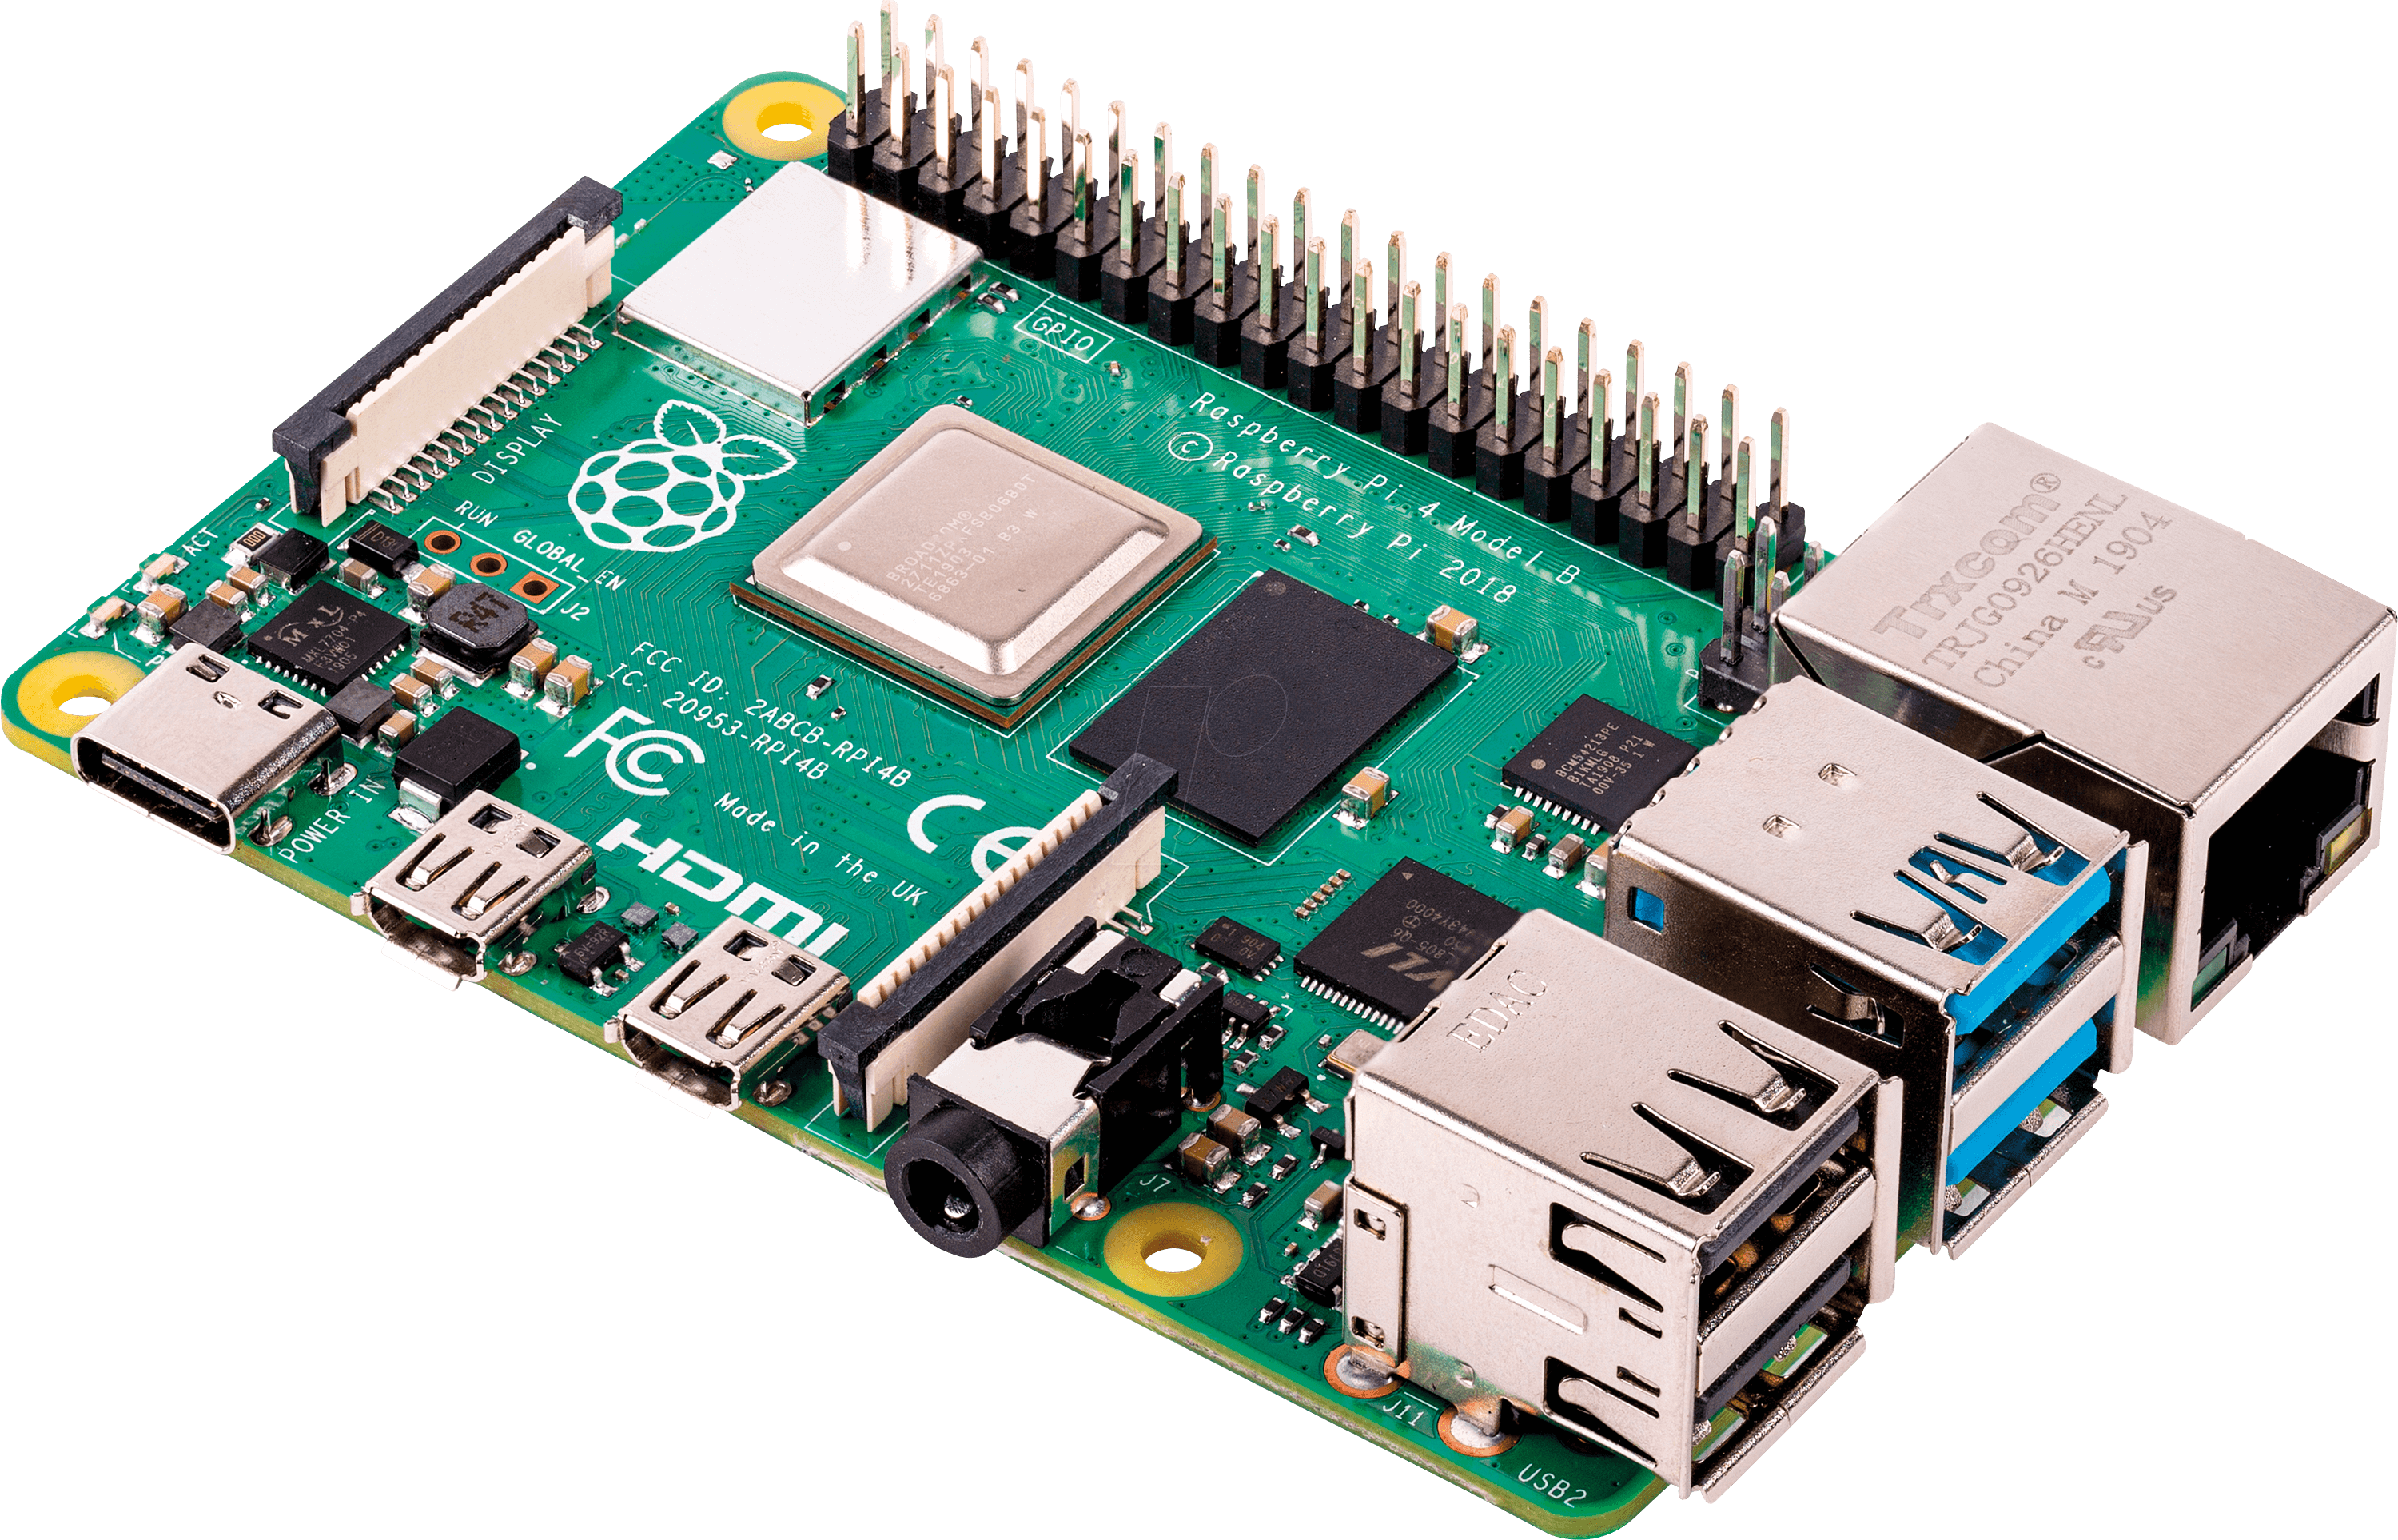
\includegraphics[width=0.4\linewidth]{photo/raspi}
\end{figure}
\end{itemize}
\end{frame}
%
%--------------------------------------------------------------------------------------------
%
\begin{frame}
\frametitle{Raspberry Pi 3B+ - Part ll}
\begin{columns}[c] % The "c" option specifies centered vertical alignment while the "t" option is used for top vertical alignment
\column{.45\textwidth} % Left column and width
\begin{itemize}
\item For our purpose, we use the Rasp- berry Pi Camera Module 8MP v2.1. It can capture pictures with 1080p and 8-megapixel focus \\
\item Connector on the Raspberry Pi 3B+ with a 15 Pin Ribbon Cable
\end{itemize}
\column{.45\textwidth} % Right column and width
PiCamera Module
\begin{figure}
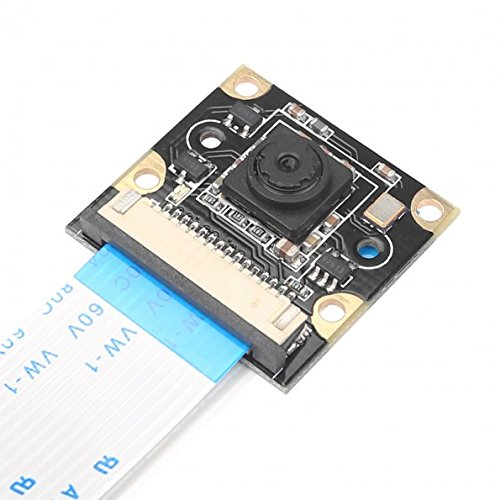
\includegraphics[width=0.7\linewidth]{photo/camera.jpg}
\end{figure}
\end{columns}
\end{frame}
%
%--------------------------------------------------------------------------------------------
%
\begin{frame}
\frametitle{Servodriver}
From SunFounder, model \textit{PCA9685}
\begin{itemize}
\item Cheap price: approximately ~13
\item Provides Pulse width modulation (PWM) to apply remote steering through the Raspberry Pi 3B+
\item Powered with 3-5V from the Raspberry Pi 3B+
\end{itemize}
\begin{figure}
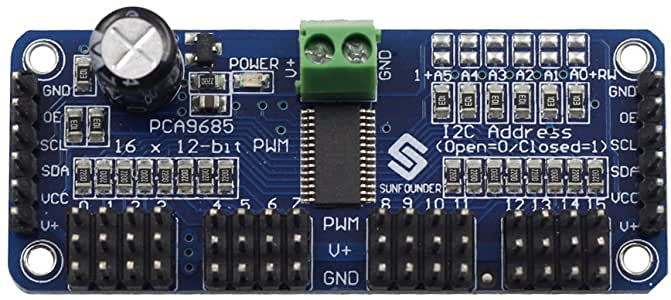
\includegraphics[width=0.4\linewidth]{photo/sunfounder.jpeg}
\end{figure}
\end{frame}
%
%--------------------------------------------------------------------------------------------
%
\begin{frame}
\frametitle{Cable Management - Part I}
\begin{block}{Raspberry Pi 3B+ to Servodriver}
8 Pin's need to be connected. 
\begin{itemize}
\item Ground GND
\item Power VCC 5 Volt
\item 2x3 Pin's for the steering and throtteling
\end{itemize}
\end{block}
\begin{block}{Servodriver to Servomotor}
Four Pin's need to be connected. 
\begin{itemize}
\item Ground GND
\item Power VCC 5 Volt
\item 2 Pin's for the steering and throtteling
\end{itemize}
\end{block}
\end{frame}
%
%------------------------------------------------------------------------------------------
%
\begin{frame}
\frametitle{Cable Management - Part ll}
\begin{figure}
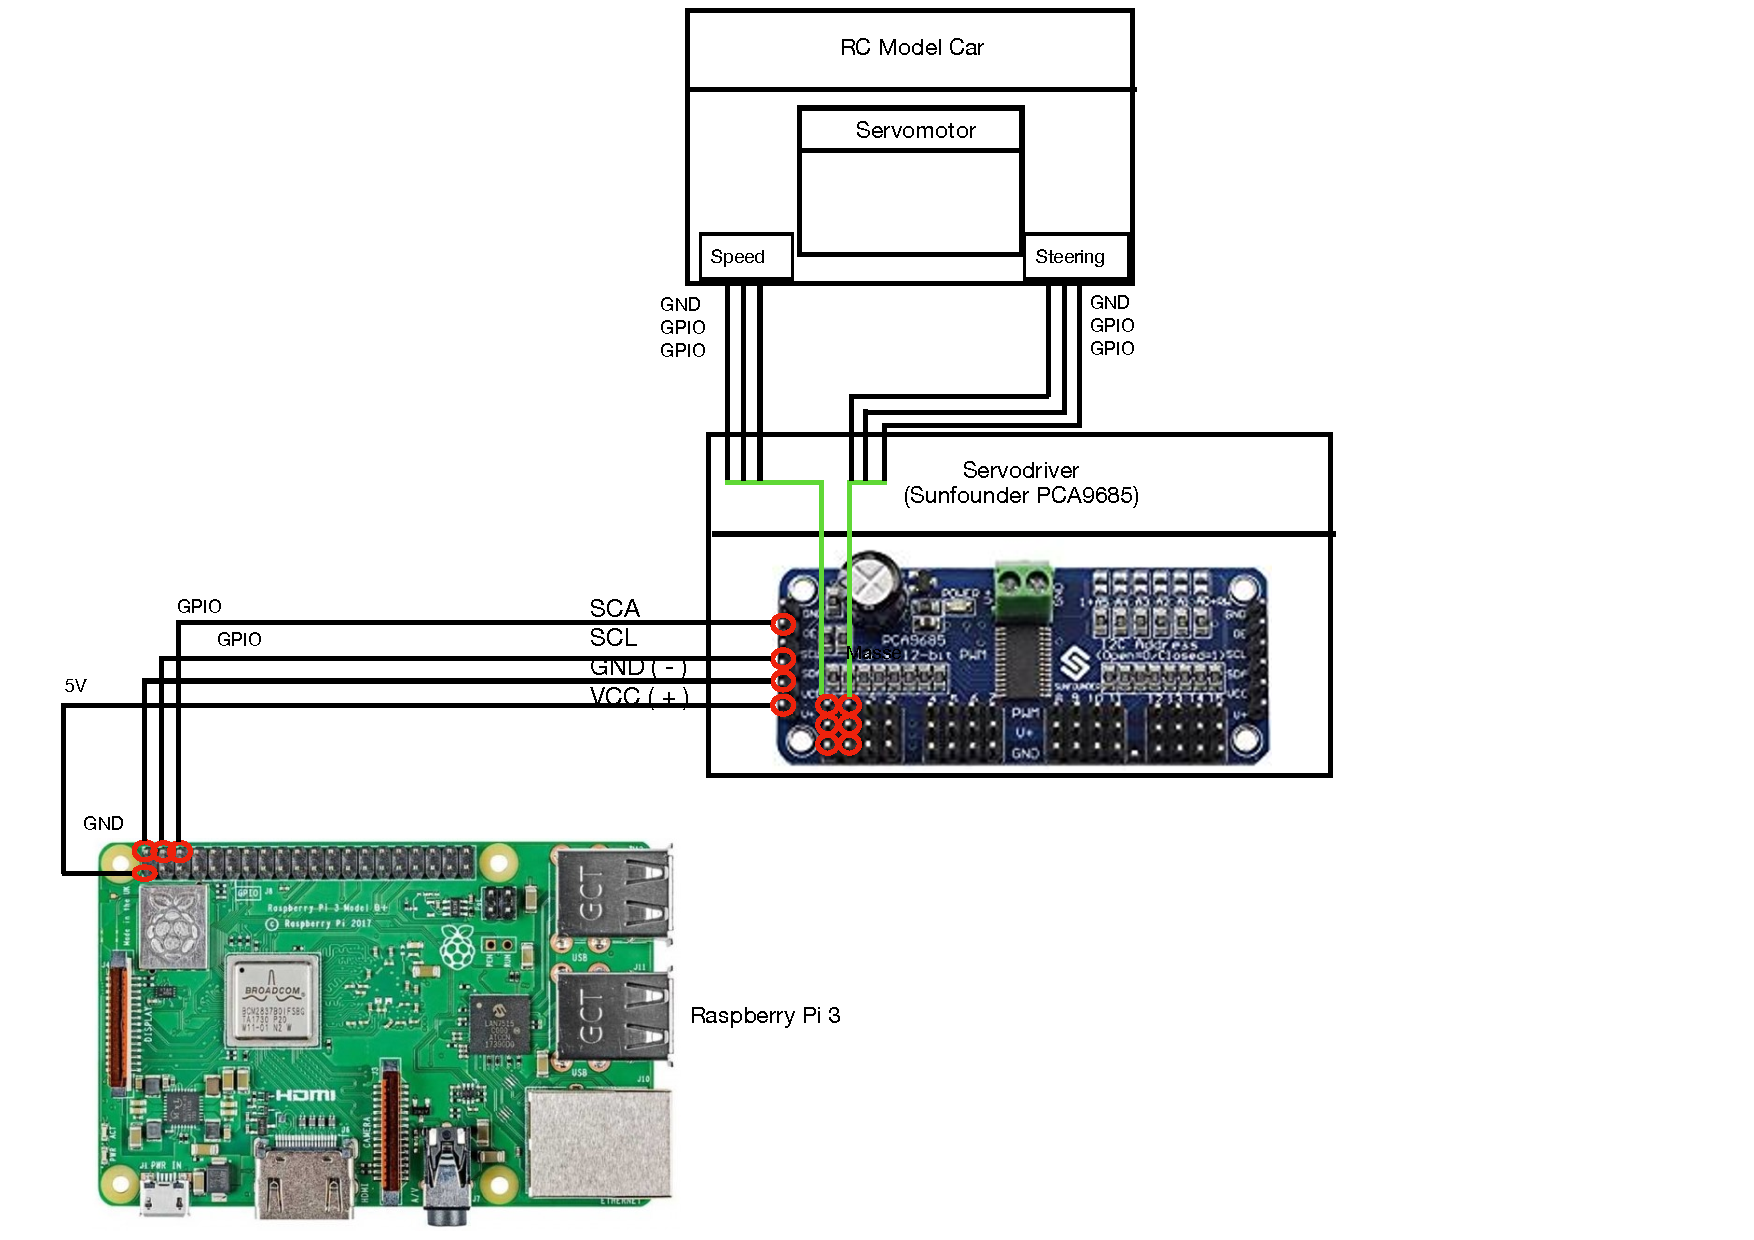
\includegraphics[width=0.7\linewidth]{photo/ebene2.pdf}
\end{figure}
\end{frame}
%
%------------------------------------------------------------------------------------
\section{Software}
%------------------------------------------------------------------------------------
%
\begin{frame}
\frametitle{Software Architecture - Python Files}
The Donkey Self-Driving Car Project is the basis for our group Project. The Filesystem is: \\
\begin{itemize}
\item Management: Start the Webserver
\item Parts: Controls the single parts, e.g. Camera, Steering, Throttle, ..
\item Templates: Web Templates for the Webserver
\item Test: Start the environment without error's
\end{itemize}
\end{frame}

%------------------------------------------------------------------------------------

%------------------------------------------------------------------------------------

\begin{frame}
\frametitle{Python Tornado Webserver}
\begin{figure}
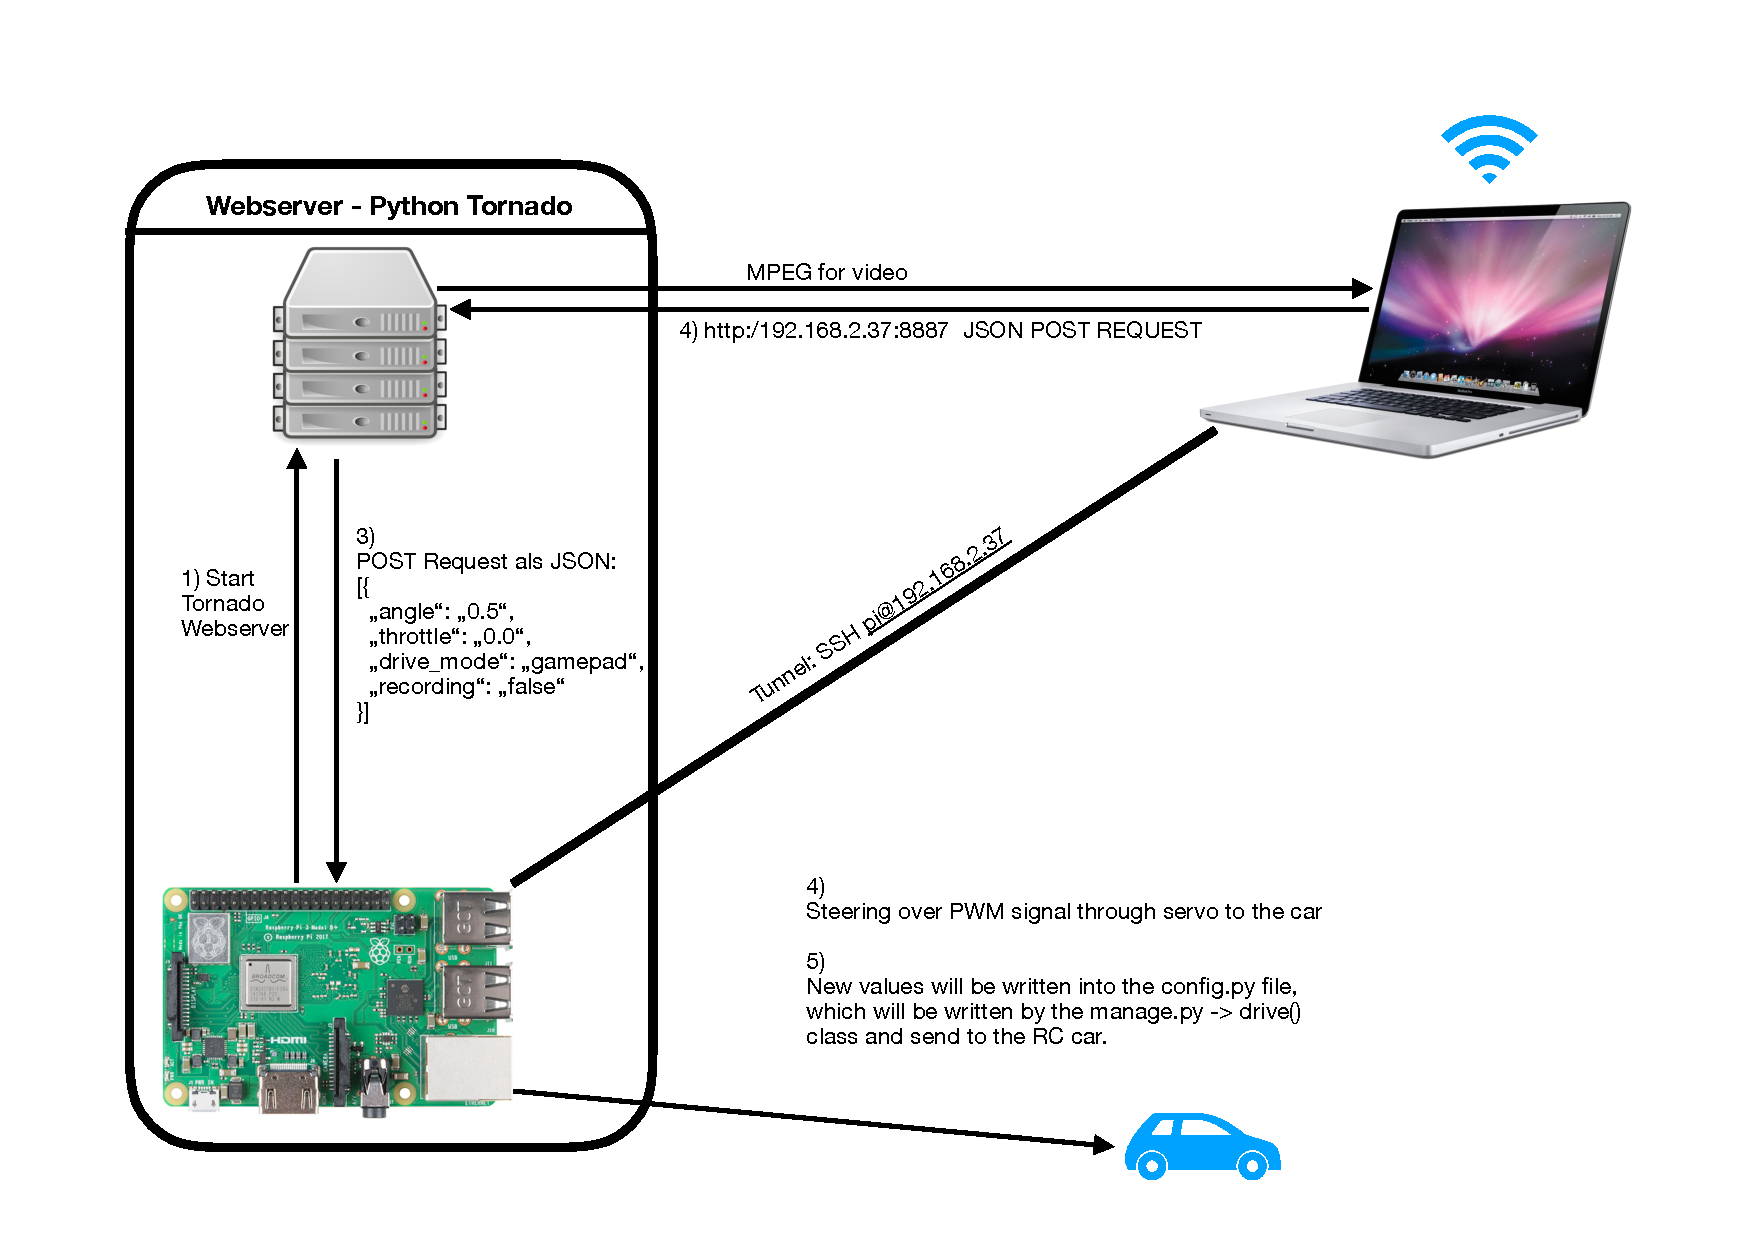
\includegraphics[width=0.9\linewidth]{photo/webserver.pdf}
\end{figure}
\end{frame}

%------------------------------------------------------------------------------------

\begin{frame}
\frametitle{Training the model with Unity}
\begin{columns}[c] % The "c" option specifies centered vertical alignment while the "t" option is used for top vertical alignment

\column{.45\textwidth} % Left column and width
\begin{itemize}
\item For capturing enough images, someone from the DonkeyCar community programmed a Unity Game.
\item Simulator of the real word with lines on the border of the track for the image recognition task
\end{itemize}

\column{.45\textwidth} % Right column and width
Snapshot from the Simulation
\begin{figure}
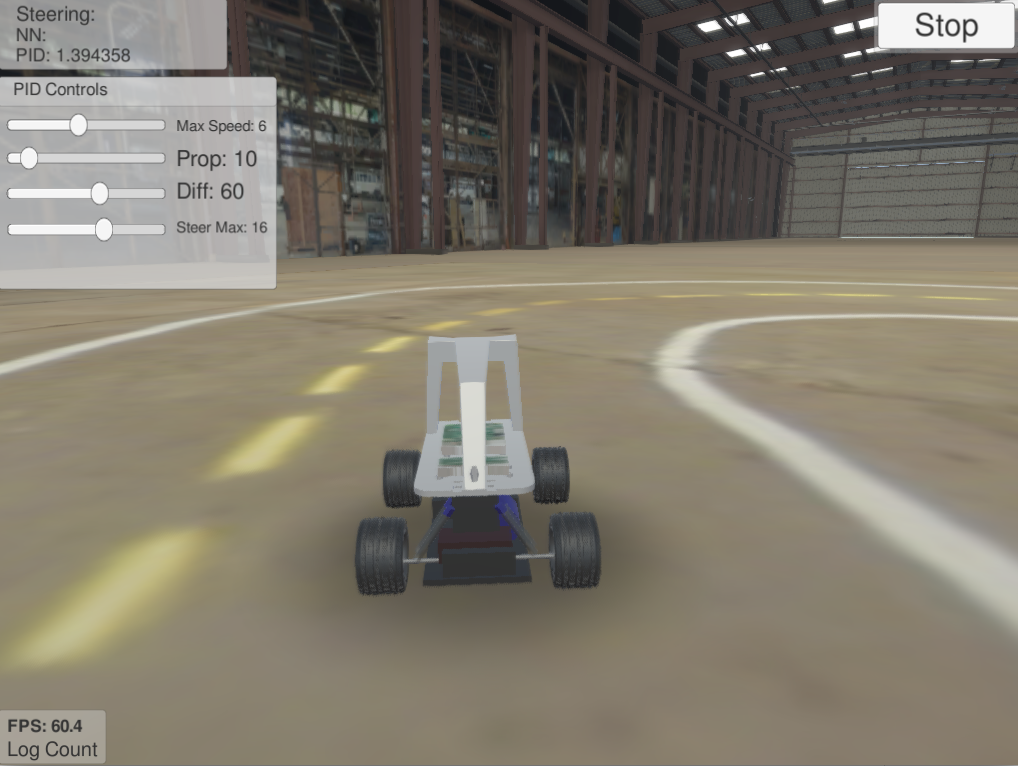
\includegraphics[width=0.9\linewidth]{photo/unity}
\end{figure}
\end{columns}
\end{frame}

%------------------------------------------------------------------------------------
\section{Machine Learning}
%------------------------------------------------------------------------------------

\begin{frame}
\frametitle{Machine Learning - Part I}
\epigraph{"A computer program is said to learn from experience E with respect to some class of tasks T and performance measure P, if its performance at tasks in T, as measured by P, improves with experience E"}{--- \textup{Mitchel }, 1979}
\end{frame}
%
%------------------------------------------------------------------------------------
%
\begin{frame}
\frametitle{Machine Learning - Part II}
\begin{itemize}
\item Casully explained: Machine Learning is a functions which could be optimized
\end{itemize}
\begin{figure}
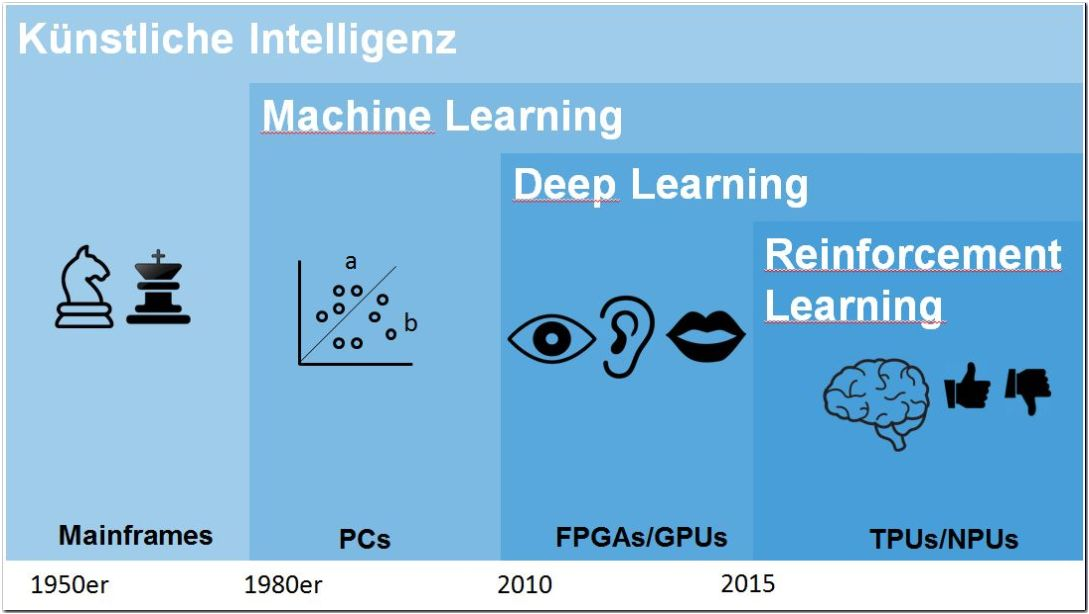
\includegraphics[width=0.8\linewidth]{photo/history}
\end{figure}
\end{frame}

%------------------------------------------------------------------------------------
%
\begin{frame}
\frametitle{Deep Learning - Part I}
\epigraph{"We get a deep neural network if we had more than one hidden layer in a neural network . Neural Networks are a concept in the machine learning discipline which try to build a program that learns like the human brain is learning."}{--- \textup{Andrew Ng }, 2013}
\end{frame}
%
%------------------------------------------------------------------------------------
%
\begin{frame}
\frametitle{Deep Learning - Part II}
\begin{columns}[c] 
\column{.45\textwidth} % Left column and width
\textbf{Parts of a Convolutional Neural Network:}
\begin{enumerate}
\item Convolutional Layers (CONV)
\item Pooling Layers (POOL)
\item Fully connected Layers (FC)
\end{enumerate}
\column{.5\textwidth} % Right column and width
\begin{figure}
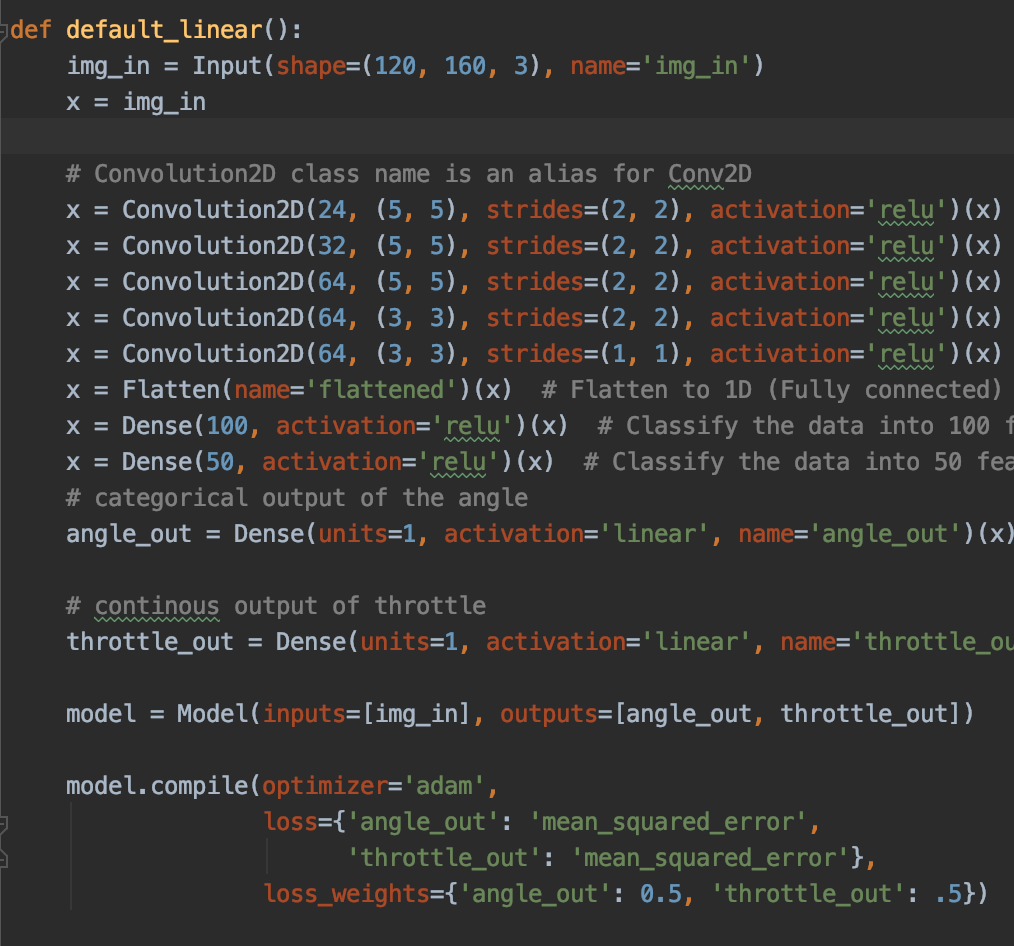
\includegraphics[width=1.05\linewidth]{photo/code.png}
\end{figure}
\end{columns}
\end{frame}
%
%------------------------------------------------------------------------------------
%
\begin{frame}
\frametitle{Deep Learning - Part III}
\begin{columns}[c] % The "c" option specifies centered vertical alignment while the "t" option is used for top vertical alignment
\column{.45\textwidth} % Left column and width
\textbf{Keyfacts of our deep Network: }
\begin{enumerate}
\item VGG16 Architecture (convolutional neural networks)
<<<<<<< HEAD
\item 266.628 Parameters
\item Based on Nvidias research 
\item The final version has a Pooling Layer (basic implementation not)
=======
\item 266.628 parameters
\item Based on Nvidias research 
\item The final version has pooling layer (basic implementaion has not)
>>>>>>> 98508cec2ff0c563ac7e8d63e0b02e834603697c
\end{enumerate}
\column{.5\textwidth} % Right column and width
\begin{figure}
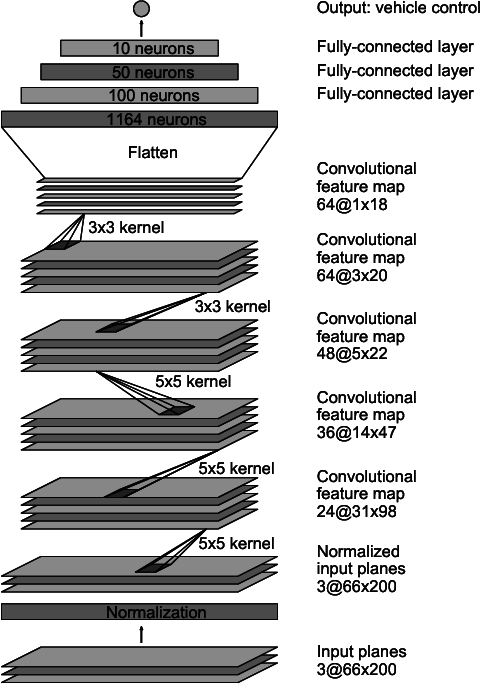
\includegraphics[width=0.75\linewidth]{photo/CNNArchitecture.png}
\end{figure}
\end{columns}
\end{frame}
%
%
%------------------------------------------------------------------------------------
\section{Autonomously Driving}
%------------------------------------------------------------------------------------
%
\begin{frame}
\frametitle{Keras Pilot - Part I}
The Keras Pilot (\textit{.h5} Format) is stored on the Raspberry Pi. 
\begin{itemize}
\item The image captured with the PiCamera are 160x120x3 Pixels
\item They pass through the follwing Neural Network
\item The Output in the last fully connected Layer is \\ (\textit{angle\_out} and \textit{throttle\_out})
\end{itemize}
\begin{figure}
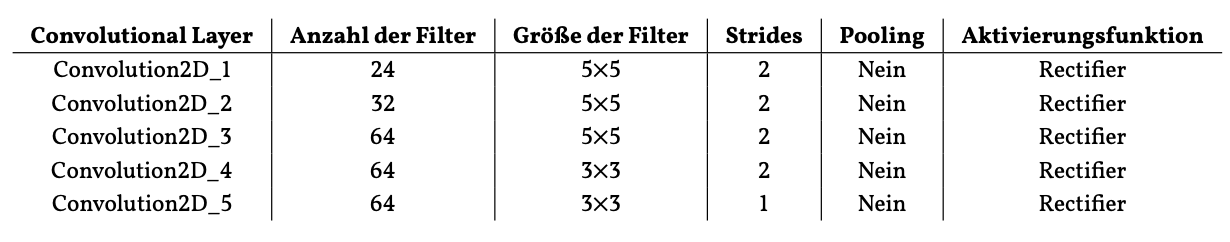
\includegraphics[width=1\linewidth]{photo/cnn_table}
\end{figure}
\end{frame}
%---------------------------------------------------------------------------------
\begin{frame}
\frametitle{Keras Pilot - Part ll}
Connection with the PiCamera Module:
\begin{columns}[c] % The "c" option specifies centered vertical alignment while the "t" option is used for top vertical alignment
\column{.45\textwidth} % Left column and width
\begin{itemize}
\item We use 20 frames per second (FPS)
\item We use Tensorflow 1.1.17 for version compatibility
\item According to that, the car changes 20 times per second the angle
\item The throttle is fix, because of the space limitation
\end{itemize}
\column{.45\textwidth} % Right column and width
\begin{center}
	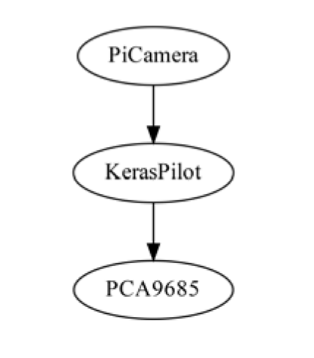
\includegraphics[width=4cm]{photo/autonom}
\end{center}
\end{columns}
\end{frame}
%----------------------------------------------------------------------------------------
\section{Evaluation}
%------------------------------------------------------------------------------------
\begin{frame}
\frametitle{Evaluation - Part l}
\begin{columns}[c] % The "c" option specifies centered vertical alignment while the "t" option is used for top vertical alignment
\column{.45\textwidth} % Left column and width
\begin{block}{Evaluation}
Even though CNN perform a really good result in the computer vision field, it is still quite hard to decompse the decisions and the filters to understand the blackbox behind. For this reason visualized one decision by plotting the occlusion maps (next page) based on this criterion function
\end{block}
\column{.45\textwidth} % Right column and width
The criterion function:
\begin{equation}
O_{i,j}= \begin{cases}
    0,& \text{if } abs(\hat{y}_{i,j} - y) > \epsilon\\
    1              & \text{otherwise} \end{cases}
\end{equation}
\end{columns}
\end{frame}
%----------------------------------------------------------------------------------------
\begin{frame}
\begin{block}{Evaluation - Part ll: Occlusion maps generated out of the CNN layers from section \textit{Autonomously Driving - Keras Pilot (Part l)}}
\begin{center}
	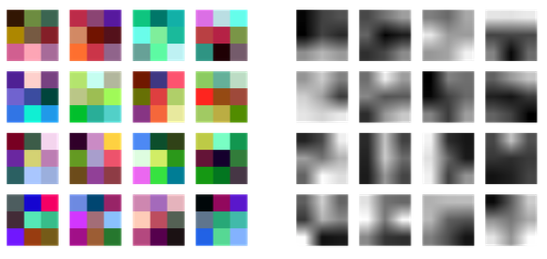
\includegraphics[width=5cm]{photo/filter}
\end{center}
\begin{center}
Not interpolated filter and gray with bilinear interpolation
\end{center}

\begin{center}
	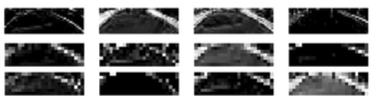
\includegraphics[width=6cm]{photo/activations}
\end{center}
\begin{center}
Activation features after each Layer of the NN respectively
\end{center}
\end{block}
\end{frame}
%------------------------------------------------------------------------------------
\begin{frame}
\frametitle{Conclusion}
\begin{block}{Final Thoughts}
The project was challenging, but all of us learned a lot during this 2 semester long process of building up this project. While doing this project, Tensorflow 2.0 was released and this changed a lot. We needed to adjust constantly, because the Tech-research is so fast.
In conclusion, we had a great time and are eager to dive deeper into Deep Learning!
\end{block}
\begin{block}{Acknowledgement}
The authors would like to thank Prof Dr. Florian Gallwitz from the University of Applied Science - Georg Simon OHM in Nuremberg.
\end{block}
\end{frame}
%
%------------------------------------------------------------------------------------
%
\begin{frame}
\frametitle{References}
\begin{itemize}
\item Github: https://github.com/bohniti/it-projekt
\item Website: https://bohniti.github.io/it-projekt/project/
\end{itemize}
\begin{block}{Sources}
All of our sources are listed in the project paper on Github.
\end{block}
\begin{center}
Thanks for listening!
\end{center}
\end{frame}
%
%------------------------------------------------------------------------------------
%
\begin{frame}
\Huge{\centerline{The End}} 
\vspace{5mm}
\begin{center}
	
\includegraphics[width=10cm]{photo/logo}
\end{center}
\end{frame}
%----------------------------------------------------------------------------------------
\end{document} 